% lang=fr
\documentclass[12pt, letterpaper, twoside]{article}
\usepackage[top=3cm, bottom=3cm, left=3cm, right=3cm]{geometry}
\usepackage[fleqn]{amsmath}
\usepackage{amssymb}
\usepackage{tikz}
\usetikzlibrary{arrows}
\usetikzlibrary{shapes,decorations}
\usepackage{comment}

\usepackage[utf8]{inputenc}
\usepackage[T1]{fontenc}
\usepackage[french]{babel}

\usepackage{lmodern}
\usepackage{caption}
\captionsetup[figure]{labelformat=empty}

\title{Projet : réponses}
\author{Lomàn Vezin \\ Raphaël Vock}

\newcommand{\T}[1]{\texttt{#1}}
\newcommand{\V}[0]{\texttt{Vector3D}}
\newcommand{\double}{\texttt{double}}

\usepackage{hyperref}

\usepackage[utf8]{inputenc}
\usepackage[T1]{fontenc}
\usepackage{microtype}
\DisableLigatures[>]{encoding = T1}

\usepackage{graphicx}

\def\O{\mathcal{O}}
\def\epsilon{\varepsilon}

\renewcommand{\familydefault}{\sfdefault}
\begin{document}
\maketitle
\section{La classe \T{Vector3D}}
\subsection{Conception}
\noindent \textbf{(P1.1)} Les points et vecteurs de l'espace euclidien sont représentés au moyen de la classe \V\ dont les attributs \T{x}, \T{y}, \T{z} (de type \double) représentent les coordonnées cartésiennes d'une instance. Celles-ci sont des attributs privés, mais tout le reste est publique. Voici les opérations que nous avons implémentées en premier :

\begin{itemize}

\item \T{getCoords()} est une méthode qui retourne les coordonnées d'une instance via un \T{std::array<double,3>}.

\item \T{norm()} et \T{norm2()} retournent la norme euclidienne (resp. norme euclidienne au carré).

\item \T{distance(x,y)} et \T{distance2(x,y)} sont des méthodes statiques qui retournent la distance euclidienne (resp. distance euclidienne au carré) entre deux \T{Vector3D} passés en argument.

\item \T{unitary()} est une méthode qui retourne le vecteur unitaire de même sens et de même direction (et lance une exception si l'instance est le vecteur nul ; voir point suivant).

\item \T{is\_zero()} est une méthode qui retourne un booléen indiquant si l'instance est plus petite (en norme au carré) qu'une (petite) constante de classe \T{EPSILON} de type \double.
\end{itemize}

\subsection{Constructeur, constructeur de copie}
\noindent \textbf{(P4.1)} L'unique constructeur de la classe prend en argument trois \double\ (nuls par défaut) et initialise un \V\ avec les coordonnées cartésiennes précisées. En l'absence d'attributs pointeurs, le constructeur de copie minimal par défaut réalise exactement ce que l'on attend, donc \textbf{nous n'avons pas défini de constructeur de copie.}

\subsection{Coordonnées sphériques}
\noindent \textbf{(P4.2)} \textbf{Nous n’avons pas implémenté de constructeur en coordonnées sphériques.} Avant tout, l’ajout de ce dernier serait un peu technique au niveau du prototypage de car nous aurions \textit{a priori} deux constructeurs aux protoypes identiques. Ce n'est pas un problème incontournable ; on pourrait, par exemple, écrire un seul et unique constructeur dont le quatrième argument est un \T{bool} (\T{false} par défaut) qui précise si les arguments donnés doivent être compris comme des coordonnées sphériques ou sinon cartésiennes.

Mais le problème fondamental est le suivant : un repère sphérique est intextricablement lié à la donnée d'un point $O$ considéré comme l'origine. Pour écrire un constructeur sphérique sans ambiguité il serait donc nécessaire :
\begin{itemize}
\item ou bien de faire un choix canonique de $O$ qui ne changerait pas du début à la fin
\item ou bien de préciser $O$ en le passant comme argument.
\end{itemize}
Si l'on choisit la première option, l'unique avantage des sphériques serait perdue car on ne serait plus en mesure de choisir l'origine à notre gré pour simplifier, entre autres, des expressions de force (e.g. en choisissant $O$ l'origine d'un champ de force central). Mais la deuxième option serait coûteuse à implémenter et lourde à utiliser, pour des avantages qui, selon nous, n'en vaudraient pas le coup.

\subsection{Surcharge des opérateurs}
\noindent \textbf{(P4.3)}
\begin{itemize}
\item Nous avons surchargé les opérateurs d'auto-affectation \T{+=}, \T{-=}, \T{*=} correspondant à l'addition (resp. soustraction) vectorielle et la multiplication par un scalaire. Celles-ci retournent le résultat de l'affectation pour optimiser certains calculs par la suite.

\item À partir de ces derniers nous avons surchargé les opérateurs binaires \T{+}, \T{-}, \T{*} correspondant aux opérations vectorielles usuelles.

\item Les opérateurs binaires \T{|} et \T{$\wedge$} retournent respectivement le produit scalaire euclidien et le produit vectoriel.

\item L'opérateur de comparaison \T{==} est défini à partir de la méthode \T{is\_zero()} (cf. \S1.1). L'opérateur \T{!=} retourne la négation logique de \T{==}.

\item L'opérateur d'indexage \T{[]} est surchargé pour permettre un accès direct (mais protégé) à chaque coordonnée sans devoir passer par \T{getCoords()} (cf. \S 1.1). Ainsi \T{u[0]}, \T{u[1]}, \T{u[2]} retourne une \textit{copie} de \T{x}, \T{y}, \T{z} respectivement. Une exception est bien-sûr lancée si l'indice n'est pas \T{0}, \T{1} ou \T{2}.
\end{itemize}

\section{La classe \T{Particle}}

\subsection{Facteur gamma, énergie}
\noindent \textbf{(P5.1)}
L'implémentation du facteur gamma et de l'énergie dans la classe \T{Particle} peut être accomplie par un attribut ou par une méthode. Chacun présente des avantages et des inconvénients.

\begin{itemize}

\item \textbf{Sous forme d'attribut:}
\subitem $\oplus$ Leur valeur serait calculée une et une seule fois, donc une même valeur ne serait jamais calculée deux fois inutilement.
\subitem $\ominus$ Leur valeur devrait être calculée systématiquement à chaque mise-à-jour de l'instance. Donc eventuellement même si elle ne servira jamais.
\subitem $\ominus$ Rajouter des attributs, c'est augmenter le poids des instances.

\item \textbf{Sous forme de méthode:}
\subitem $\oplus$ La masse et la vitesse sont des grandeurs \textit{essentielles} d'une particule tandis que le gamma et l'énergie en découlent via des fonctions mathématiques. Conceptuellement, les attributs d'une classe devraient être reservées aux variables \textit{libres} et les méthodes aux variables \textit{liées}.

\subitem $\oplus$ Stockées sous forme de méthodes, on calcule leur valeur précisément lorsqu'on en a besoin, donc on ne stocke jamais d'information redondante.

\subitem $\ominus$ \ldots quitte à éventuellement effectuer plusieurs fois le même calcul.
\end{itemize}
\bigskip
\textit{A priori} ses grandeurs seront accédés plusieurs fois par mise à jour de l'accélérateur. C'est pourquoi nous avons décidé de les implémenter sous forme d'attribut.

\section{Premiers éléments}

\subsection{Les éléments en général}
\noindent \textbf{(P6.1)} Dans la hiérarchie des classes représentant les divers éléments de l'accélérateur, nous avons mis comme nœud une classe abstraite nommée \T{Element} dont les attributs représentent les paramètres purement géométriques (points d'entrée et de sortie, rayon, paramètre de courbure) et relationnels (l'addresse de l'élément suivant, une liste des addresses des \T{Particle} contenues dans l'instance) des éléments. Nous considérons les éléments comme \textit{a priori} courbes, en sachant qu'on peut prendre une courbure nulle et l'instance dégénère en un élément droit. Nous définissons entre autres une méthode virtuelle pure \T{apply\_lorentz\_force(Particle \&p, double dt)} pour mettre en œuvre les intéractions élément-particule ; son comportement est délégué aux sous-classes suivantes:

\begin{itemize}
\item \T{Electric\_element} est une sous-classe d'\T{Element} avec un attribut supplémentaire, un champ de électrique \T{E} (dont nous discuterons de la représentation au passage suivant). Ainsi nous spécialisons la méthode \T{apply\_lorentz\_force(Particle \&p)} en évaluant le champ vectoriel \T{E} au point où se trouve $\T{p}$ et en incrémentant la force résultante de \T{p} via la relation $\boldsymbol{\mathrm{F}}=q\boldsymbol{\mathrm{E}}$.

\item \T{Magnetic\_element}, quant à elle, a comme attribut supplémentaire un champ magnétique \T{B}. Dans ce cas nous spécialisons \T{add\_lorentz\_force(Particle \&p)} en évaluant $\T{B}$ en $\T{p}$ puis en appliquant la méthode relativiste $$\T{Particle::add\_magnetic\_force(const Vector3D \&B, double dt)}$$ déclarée auparavant dans \T{particle.h}.

\end{itemize}

\ \linebreak
\textbf{(P6.2)} Comment représenter les champs magnétiques ?

Comme expliqué ci-dessus, les champs magnétiques sont des méthodes virtuelles pures qui prennent en argument un point de l'espace, et retournent la valeur du champ vectoriel en se point.

\ \linebreak
\ \linebreak
\textbf{(P6.3)} Afin d'alléger par la suite le corps de certaines méthodes, \textbf{nous avons implémenté le calcul du centre de courbure} avec la méthode \T{Element::center(void)}. Celui-ci n'a de sens que si la courbure est non nulle (i.e. l'élément est courbe) donc une exception est lancée dans le cas contraire.

\ \linebreak
\textbf{(P6.4)} La relation d'appartenance entre une particule et l'élément dans lequel elle se trouve se manifeste par un attribut \T{Element* current\_element}. Ceci implique directement qu'une particule ne peut appartenir qu'à un et un seul élément.

\section{La classe \T{Accelerator}}

\subsection{Généralités}
\noindent \textbf{(P7.1)} Un accélérateur \textit{est} une collection d'éléments donc nous faisons hériter la classe \T{Accelerator} de \T{std::vector<std::unique\_ptr<Element>>}. Nous passons par des \T{unique\_ptr} pour obtenir un comportement polymorphe des éléments. Par ailleurs, cette héritage est \T{private} pour rester en accord avec la norme C++.

Énumérons les principaux attributs et méthodes de cette classe :
\begin{itemize}
	\item L'attribut \T{std::vector<std::unique\_ptr<Particle>> particles} stockera les particules contenues dans l'accélérateur. Nous utilisons à nouveau des \T{unique\_ptr} pour pouvoir avoir un comportement polymorphe si le besoin se présente.
	\item L'attribut \T{const Vector3D origin} définit un point de repère sur l'accélérateur et servira à faciliter la construction de l'accélérateur.
	\item L'attribut \T{double length} décrit la longueur géométrique de l'accélérateur. Celui-ci aidera à définir un système de coordonnées curviligne global sur la longeur de l'accélérateur.
	\item La méthode \T{void addParticle(const \&Particle)} permet d'insérer une particule dans l'accélérateur \textit{tout en conservant la nature de l'instance s'il s'agit d'une sous-classe.}
	\item Pour chaque sous-classe concrète \T{E} de \T{Element} nous avons une méthode \T{addE} permettant d'ajouter une instance de cette sous-classe à l'accélérateur. Cette méthode prend en arguments un point de l'espace ainsi que les divers paramètres géométriques et physiques de l'élément en question. L'unique point correspond au point de sortie de l'élément ; le point d'entrée est déduit comme étant le point de sortie du précédent (ou sinon \T{origin} s'il n'y en a pas).
	\item La méthode \T{weld} permet de ``souder'' les éléments de l'accélérateur entre eux, i.e. d'affecter les valeurs de \T{next\_element} et \T{previous\_element}.

	\item La méthode \T{void evolve(double dt)} provoque la mise à jour de l'accélérateur en appelant la mise à jour de ses composante.
\end{itemize}

\ \linebreak
\noindent \textbf{(P7.2)} Nous supprimons le constructeur de copie par défaut ainsi que l'opérateur d'affectation \T{=} de la classe \T{Accelerator} afin de garantir l'intégrité des ses données. Ils seraient de toute façon implicitement supprimés du fait de l'existence d'attributs de type \T{unique\_ptr}, mais nous souhaitons affirmer leur suppression indépendamment des choix d'implémentation.

\subsection{Révision des éléments}

\noindent \textbf{(P8.1)} La méthode \T{has\_collided()} de la classe \T{Element} doit se comporter de façon différente si elle est appelée sur un élément courbe ou sur un élément droit. Dans une première approche il s'agirait donc en terme de programmation orientée objet d'une méthode virtuelle. Toutefois pour l'unité mathématique et conceptuelle nous regroupons ces deux cas en un seul.

\ \linebreak
\noindent \textbf{(P8.2)} On s'attendrait ainsi que la classe \T{Element} soit abstraite.

\section{Conception du système}

\subsection{Objets dessinables}

\ \linebreak
\noindent \textbf{(P9.1)} La méthode \T{draw()} a un comportement différent selon la nature de l'instance. De plus, on ne saurait la définir dans le cas général. Il s'agit donc d'une méthode virtuelle pure.

\ \linebreak
\noindent \textbf{(P9.2)} Pour obtenir dans les deux cas un comportement polymorphes, nous utilisons des listes hétérogènes à la fois de particules et d'éléments. Plus particulièrement, nous utilisons des \T{std::vector} de \T{std::vector}.

\ \linebreak
\noindent \textbf{(P9.3)} Nous devons à présent être vigilants vis-à-vis du constructeur de copie et l'opérateur d'affectation, du fait que cette classe contient des pointeurs. Une solution serait de définir une copie profonde et non de surface. Toutefois la copie d'accélérateur n'est pas une fonctionnalité qu'on envisage dans le cadre du projet, donc nous contentons de supprimer ces derniers.

\section{La classe \T{Beam}}
\noindent \textbf{(P11.1)} Les attributs de \T{Beam} (faisceau) sont les suivants :
\begin{itemize}
	\item Un tableau dynamique de \T{unique\_ptr<unique\_ptr<Particle>>}. En effet, nous voyons les faisceaux non comme des listes particules, mais des listes de références vers des particules (et donc, par souci de polymorphisme, une liste de références vers des références de particules).
	\item Un attribut \T{std::unique\_ptr<Particle>} correspondant à la \textit{particule modèle} du faisceau. De nouveau, nous utilisons un pointeur par souci de polymorphisme.
	\item L'attribut \T{double lambda} correspondant au facteur de proportionnalité entre la particule modèle et les particules qui seront effectivement construites.
	\item L'attribut \T{uint N} correspondant au nombre de particules qui seront construites dans l'accélérateur.
	\item L'attribut \T{Accelerator* habitat} correspond à l'accélérateur dans lequel le faisceau évolue. Cet attribut est nécessaire car certaines méthodes dépendent intimement de la géométrie de l'accélérateur en question.
	\item Les divers renseignements physiques (énergie, coefficients elliptiques) sont donnés sous forme de méthodes.
\end{itemize}

\section{Interactions inter-particules}
\subsection{Première approche}
\noindent \textbf{(P13.1)} Étant donnée une collection de $n$ il y a $1+2+\cdots+n = n(n+1)/2$ interactions qui ont lieu. Ceci donne lieu donc à un un algorithme en $\O(n^2)$ dans les deux cas.

\subsection{Meilleure voisins}
\noindent \textbf{(P14.1)} Notons à nouveau $n$ le nombre de particules, et $k$ le nombre de cases. Si l'on suppose que les particules sont équi-réparties dans les cases, alors chaque case contient $n/k$ particules. Avec un même raisonnement que ci-dessus, la complexité temporelle du calcul d'évolution de chaque case est donc $\O((n/k)^2)$, soit $\O(n^2)$ si on considère $k$ comme fixé. En sommant donc sur les cases on obtient donc une complexité globale qui est de nouveau en $\O(n^2)$ (bien que la constante est \textit{a priori} sensiblement plus faible qu'avec l'algorithme naïf).

Il y a trois inconvénients à cet algorithme:
\begin{itemize}
	\item \textit{Une perte de précision.} les interactions ne tiennent compte que d'un petit voisinage autour de la particule, correspondant à la taille de la case.
	\item \textit{Une complexité peu intéressante.} Elle croit quadratiquement avec le nombre de particules.
	\item \textit{Un algorithme qui ne tient pas compte de la répartition des particules.} Si, admettons, les particules ne sont pas équi-réparties dans l'accélérateur, l'échantillonnage de l'espace ne s'adapte pas pour tenir compte de leur déséquilibre.
\end{itemize}

\noindent \textbf{(P14.2)} Au vu des inconvénients présentés ci-dessus, l'algorithme proposer n'est pas celui qui figure dans le programme. En implémentant une version modifiée de l'algorithme de Barnes-Hut, nous sommes arrivés à une précision supérieure tout en ayant une complexité temporelle moyenne en $\O(n \log n)$ Nous détaillons son implémentation dans l'annexe.

\newpage

\part*{Extensions}
\section{Algorithme de Barnes--Hut}
Comme énoncé plus haut, le schéma de gestion des voisins est un algorithme subquadratique basé sur l'approximation de Barnes--Hut.
\subsection*{Cadre et motivation}
L'algorithme de Barnes--Hut\footnote{\url{https://en.wikipedia.org/wiki/Barnes-Hut_simulation}} est conçu pour simuler de façon efficace le problème à $n$ corps gravitationnel, non relativiste. En toute généralité, on peut l'adapter dans le cadre plus général d'un système de champs de force centrale (qui décroit rapidement avec la distance) engendrés par $n$ particules qui interagissent toutes entre elles.

Donnons l'idée avec un exemple : supposons que l'on dispose de trois particules A, B et C qui interagissent entre elles. (Pour fixer les idées dans le cadre du projet, disons que cette interaction est de nature électromagnétique). Supposons que A et B sont proches l'une de l'autre, mais que C est loin de ces dernières. Pour calculer l'influence de A et B sur C, on imagine qu'à une bonne approximation on puisse se contenter de ``moyenner'' A et B en une particule ``virtuelle'' P, puis de calculer l'influence de P sur A. Concrètement, pour effectuer cette moyenne, on choisit la grandeur inertielle pertinente selon la nature de la force (donc dans ce cas-là la charge, mais pour la gravité on utiliserait la masse) et on calcule le barycentre de A et B, pondéré par cette grandeur.

Ainsi on arrive à réduire le nombre de calculs de force via un processus de moyennage. L'idée est de cumuler ces moyennages afin d'obtenir une complexité globalement plus faible via un algorithme de recherche transverse dans un arbre.

\subsection*{La structure de donnée pertinente}
On va considérer une structure de données correspondant à un découpage récursif de l'espace en pavés. On part d'un pavé peuplé d'un certain nombre de particules. S'il contient au moins deux, on le découpe en $2^3 = 8$ sous-pavés égaux. Sur chaque sous-pavé contenant au moins une particule on répète ce processus, et ainsi de suite jusqu'à que chaque particule occupe son propre pavé.

En pratique, on procédera plutôt dans l'autre sens : en partant d'un arbre vide, on insère les particules une à une en en suivant le même algorithme. (Dans la littérature anglo-saxonne on utilise le terme le terme \textit{octree}. Dans le code, il s'agit de la classe \T{Node}.) À chaque insertion d'une particule dans un pavé on met à jour la ``particule barycentrique'', qui permettra par la suite les calculs de force.

\subsection*{Description du calcul de force}
Lorsqu'il s'agit de calculer l'interaction totale d'un ensemble de particules stockées sous la forme d'un arbre A sur une particule donnée C, on traverse l'arbre selon l'algorithme suivant :

\begin{enumerate}
	\item Si le pavé ne contient pas de particule, il n'y a rien à faire.
	\item S'il contient 1 particule, on fait agir cette unique particule sur A.
	\item Sinon, on calcule le rapport du volume du pavé correspondant à C par le cube de la distance séparant A de la particule barycentrique de A.
\begin{itemize}
	\item Si ce rapport est suffisamment petit (disons plus petit qu'un paramètre adimensionné $\theta$ correspondant à la précision de la simulation) alors on fait agir la particule barycentrique sur A.
	\item Sinon, on répète le processus sur chaque sous-pavé.
\end{itemize}
\end{enumerate}
En d'autre termes, en partant de sa racine, on va descendre dans l'arbre jusqu'à que les distances soit suffisamment grandes qu'on puisse appliquer l'approximation barycentrique.
\subsection*{Complexité temporelle}
Si on note $\epsilon$ la distance minimale entre deux particules, alors la création de l'arbre avec $n$ particules est en $\O(n \log(1/\epsilon))$. Si les particules sont assez bien réparties on peut supposer que $\epsilon \propto 1/n$, donc on obtient finalement une complexité en $\O(n \log n)$.

Dans le cas général, lors du calcul de l'action de l'arbre sur une particule, la profondeur typique sera en $\O(\log n)$. Si les calculs algébriques sur les vecteurs sont $\O(1)$, le calcul de la force de l'arbre sur une particule donnée sera donc $\O(\log n)$. Le calcul total de toutes les interactions sera donc $\O(n \log n)$.

Ainsi, avec un tel algorithme, la méthode \T{evolve} sera $\O(n \log n) + \O(n \log n)$ soit $\O(n \log n)$.

Par la pratique, on constate qu'on est désormais capable d'augmenter le nombre de particules d'un facteur 10 à 20 par rapport à l'algorithme naïf (quadratique).

\subsection*{Précision et choix de $\theta$}
Le facteur $\theta$ quantifie la précision de l'approximation : plus il est grand, plus l'approximation est agressive mais moins elle est précise. Quand $\theta = 0$ l'algorithme dégénère en l'algorithme naïf. En mettant $\theta = 0.5$ nous avons obtenu une bonne précision sur des périodes de temps raisonnables, tout en ayant une complexité temporelle beaucoup plus intéressante.

\begin{figure}
	\centering
	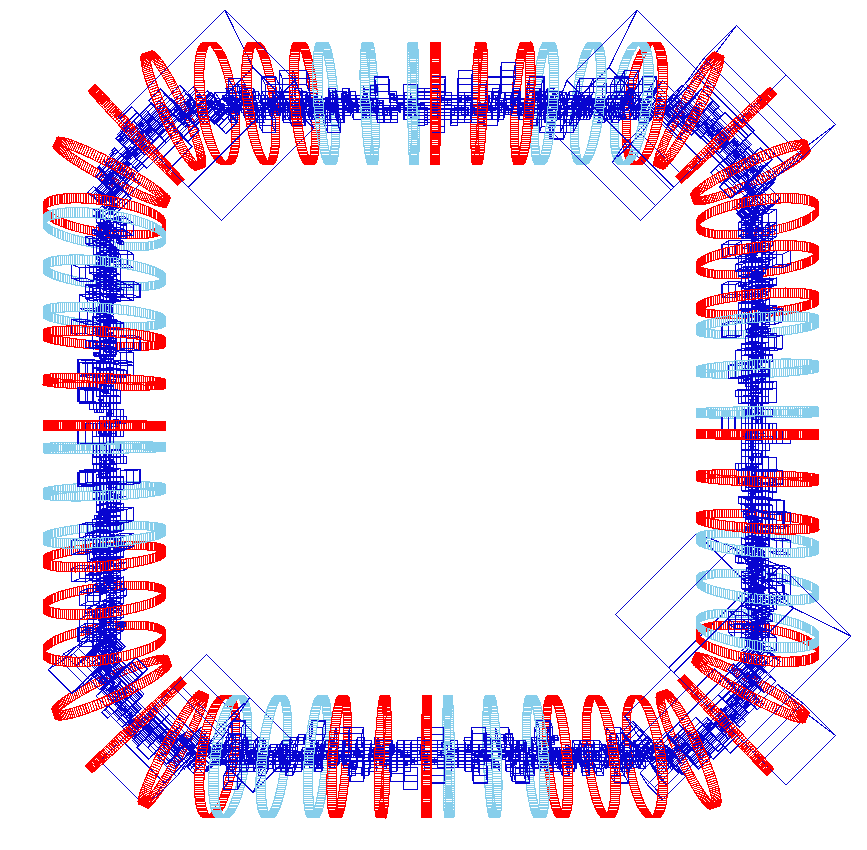
\includegraphics[width=5in]{images/octree.png}
	\caption{\textbf{Figure 1.} Visualisation des octree avec 3,000 particules}
\end{figure}

\end{document}
